%------------------------------------------------------------------------
\hypertarget{cv:eliminarCondicion}{\section{Eliminar Pre/Postcondición}} \label{sec:eliminarCondicion}

	Esta funcionalidad le permitirá eliminar una precondición innecesaria o incorrecta. 

		\subsection{Procedimiento}

			%Pasos de procedimiento
			\begin{enumerate}
	
			\item Oprima el botón \IUBotonEliminar{} de un registro existente de la pantalla \ref{fig:GestionarPrePostcondiciones} ''Gestionar Pre/Postcondiciones''.
	
			\item Se mostrará el mensaje \ref{fig:confirmaEliminaPrePost} sobre la pantalla \ref{fig:GestionarPrePostcondiciones} ''Gestionar Pre/Postcondiciones''.
			
			%Pantalla
			\begin{figure}[htbp!]
				\begin{center}
					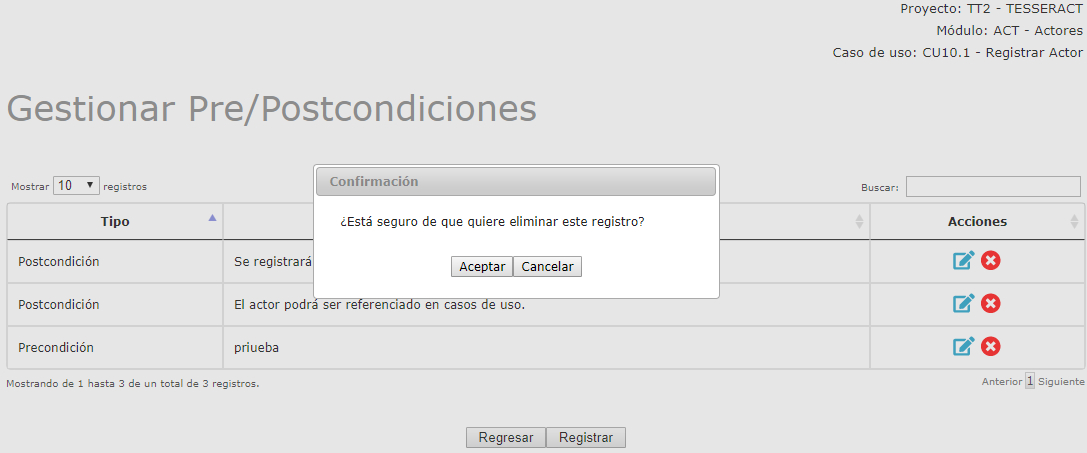
\includegraphics[scale=0.6]{roles/lider/casosUso/precondiciones/pantallas/IU6-1-2-3MSG10}
					\caption{MSG de Confirmación}
					\label{fig:confirmaEliminaPrePost}
				\end{center}
			\end{figure}
						
			\item Oprima el botón \IUAceptar.
			
			\item Se mostrará el mensaje \ref{fig:PrePostEliminada} en la pantalla \ref{fig:GestionarPrePostcondiciones} ''Gestionar Pre/Postcondiciones''.
			
			\begin{figure}[htbp!]
				\begin{center}
					
\includegraphics[scale=0.6]{roles/lider/casosUso/precondiciones/pantallas/IU6-1-2-3MSG1}
					\caption{MSG: Precondición Eliminada}
					\label{fig:PrePostEliminada}
				\end{center}
			\end{figure}
			\end{enumerate}